\documentclass[10pt,a4paper]{amsart}
\usepackage[margin=19mm]{geometry}
\usepackage{amsmath,amssymb,mathtools}
\usepackage[scr=rsfs,cal=euler]{mathalfa}
\usepackage{xfrac}
\usepackage[unicode,hidelinks,bookmarks=false]{hyperref}
\newcommand{\ie}{i.e.\ }
\newcommand{\cf}{cf.\ }
\newcommand{\resp}{respectively\ }
\newcommand{\Subsection}{\subsection}
\providecommand{\nobreakdash}{\nobreak\hbox{-}}
\setlength{\emergencystretch}{2em}
\multlinegap0pt
\usepackage{tikz}
\usepackage{amssymb}
\usepackage{float}
\usepackage[shortlabels]{enumitem}
\newtheorem{prop}{Proposition}
\newtheorem{theorem}{Theorem}
\DeclareMathOperator{\F}{F}
\DeclareMathOperator{\M}{M}
\newcommand{\hook}{\text{hook}}
\DeclareMathOperator{\m}{m}
\title{On the Smallest Partition Associated to a Numerical Semigroup}
\author{Nathan Kaplan, Kaylee Kim, Cole McGeorge, Fabian Ramirez, Deepesh Singhal}
\date{Source: arXiv:2507.04169v2 (CC BY 4.0)}
\begin{document}
\maketitle

\noindent\emph{Source and licence.} On the Smallest Partition Associated to a Numerical Semigroup. Version arXiv:2507.04169v2 (CC BY 4.0), distributed by arXiv under the Creative Commons Attribution 4.0 International licence, http://creativecommons.org/licenses/by/4.0/, as recorded in the arXiv licence metadata for this exact version and shown on the abstract page https://arxiv.org/abs/2507.04169v2. Full licence notice: \texttt{licenses/arxiv-2507.04169-CC-BY-4.0.txt}.\par\smallskip

\noindent\textit{Editorial scope.} Counted unit: the article's theorem durfee (source0.tex lines 1165--1171). The article's complete original proof of it is delivered with it (source0.tex lines 1172--1297, one \texttt{proof} environment of 126 lines). No mathematics is written, repaired or re-derived: the statement and the proof are the article's own lines, in the article's own notation, and no retained line is substituted or re-flowed.  Retained uncounted as the source-local context the proof needs: lines 522--530.  Nothing was omitted from any retained span, so the package carries no omission record.  No retained line contains a citation, so the wrapper carries no bibliography and no bibliography entry.  The retained lines contain the article's own diagram code, which the wrapper typesets with the standard tikz packages; no image file is delivered and the package declares no asset dependency.  Editorial formatting only, in addition: an AMS \texttt{amsart} preamble that restates the article's own declarations and macros used by the retained lines, namely the environments \texttt{prop}, \texttt{theorem} on separate counters, together with the standard packages those lines need.  The retained environments print in this document as Proposition 1, Theorem 1 in order of appearance, whereas the article prints the same items with the numbering of its own full document.  The complete native source of the article as distributed in the arXiv e-print for this exact version is bundled unchanged as \texttt{sources/181075/source0.tex}.
\begin{prop}
    \label{Element in I}
    Let $S$ be a numerical semigroup and $I$ be an order ideal of $(\M(S),\preccurlyeq)$ such that $T = S\cup I$ is a numerical set associated to $S$. 
For each $x \in I$ one of the following conditions holds:
    \begin{enumerate}
        \item $\F(S)-x\in I$, or
        \item there is an ideal triangle $(x,y,z)$ satisfied by $I$.
    \end{enumerate}
\end{prop}

\begin{theorem}
    \label{general durfee}
    Let $S$ be a numerical semigroup with depth 2 for which $\lambda(S)$ has a Durfee square of size $n$. Let $F = \F(S)$ and suppose that $F, F-\alpha_1, F-\alpha_2, F-\alpha_3,...,F-\alpha_{n-1}$ are the $n$ largest gaps of $S$ in descending order.
    
Suppose $\alpha_1,\ldots, \alpha_{n-1}$ have the property that $\alpha_i=\alpha_j+\alpha_k$ implies $j=k=i-1$.
    Then $S$ is $\lambda$-minimal.
\end{theorem}

\begin{proof}
Since the Durfee square of $\lambda(S)$ has size $n$, the Young diagram of $\lambda(S)$ can be partitioned as a disjoint union $n$ hooks. Suppose that the $n$ smallest elements of $S$ are $0<F-\beta_1<\dots<F-\beta_{n-1}$. Note that $\m(S)=F-\beta_1$. Therefore, $\lambda(S)$ is the disjoint union of the hooks 
\[
\hook(0,F),\ \hook(F-\beta_1,F-\alpha_1),\ldots, \hook(F-\beta_{n-1},F-\alpha_{n-1}).
\]
These hooks have sizes $F, \beta_1-\alpha_1,\dots, \beta_{n-1}-\alpha_{n-1}$, and therefore 
\[
|\lambda(S)|=F+\sum_{i=1}^{n-1}(\beta_i-\alpha_i).
\]
Note that $0<\alpha_1<\dots<\alpha_{n-1}<\beta_{n-1}<\dots<\beta_1<\frac{F}{2}$, where the last inequality follows from the assumption that $S$ has depth 2.
The following diagram illustrates these hooks.
\begin{center}
\begin{figure}
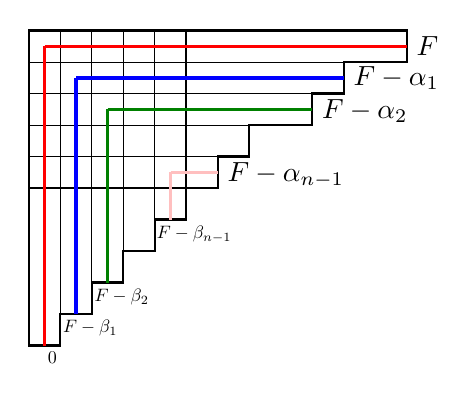
\begin{tikzpicture}[scale=0.4, x=1cm,y=-1cm]
   %---- Durfee square (3×3) ----
  \draw[thick] (0,0) rectangle (5,5);
  \foreach \i in {1,2,3,4}{
    \draw (0,\i) -- (5,\i);
    \draw (\i,0) -- (\i,5);
  }

  %---- extend the first three rows ----
  \draw (5,0) -- (12,0);  % row 1 → length 8
  \draw (5,1) -- (10,1);  % row 2 → length 6
  \draw (5,2) -- (9,2);  % row 3 → length 4
  \draw (5,3) -- (7,3);
  \draw (5,4) -- (6,4);

  %---- extend the first three columns ----
  \draw (0,5) -- (0,10);  % col 1 → height 8
  \draw (1,5) -- (1,9);  % col 2 → height 7
  \draw (2,5) -- (2,8);  % col 3 → height 5
  \draw (3,5) -- (3,7);
  \draw (4,5) -- (4,6);

  %---- full boundary of λ = (8,6,4,3,3,2,2,1) ----
  \draw[thick]
    (0,0) --
    (12,0) --(12,1) --
    (10,1) -- (10,2) --
    (9,2) -- (9,3) --
    (7,3) -- (7,4) --
    (6,4) -- (6,5) --
    (6,5) -- (5,5) --
    (5,6) -- (4,6) --
    (4,7) -- (3,7) --
    (3,8) -- (2,8) --
    (2,9) -- (1,9) --
    (1,10) -- (0,10) --
    (0,0);

  %---- labels at row‐ends ----
  \node[right] at (12,0.5) {$F$};
  \node[right] at (10,1.5) {$F - \alpha_1$};
  \node[right] at (9,2.55) {$F - \alpha_2$};
  \node[right] at (6,4.6) {$F - \alpha_{n-1}$};

  %---- labels at column‐ends ----
  \node[below,scale=0.65] at (0.75,10) {$0$};
  \node[below,scale=0.65] at (1.95,9) {$F-\beta_1$};
  \node[below,scale=0.65] at (2.95,8) {$F - \beta_2$};
  \node[below,scale=0.65] at (5.25,6) {$F - \beta_{n-1}$};

  %---- hooks ----
  \draw[red,very thick]
    (0.5,0.5) -- (12,0.5);
\draw[red,very thick]
    (0.5,0.5) -- (0.5,10);
  \draw[blue,very thick]
    (1.5,1.5) -- (10,1.5);
\draw[blue,very thick]
    (1.5,1.5) -- (1.5,9);
  \draw[green!50!black,very thick]
    (2.5,2.5) -- (9,2.5);
\draw[green!50!black,very thick]
    (2.5,2.5) -- (2.5,8);
    \draw[pink,very thick]
    (4.5,4.5) -- (6,4.5);
\draw[pink,very thick]
    (4.5,4.5) -- (4.5,6);
\end{tikzpicture}
\caption{Decomposition of Young diagram into $n$ hooks}
\end{figure}
\end{center}

We now consider the set of ideal triangles of $S$ that could potentially contain $F-\alpha_i$. Suppose $(F-\alpha_i,u,v)$ is an ideal triangle of $S$. Then $F-v$ is a gap of $S$ and $F>F-v=(F-\alpha_i)+u>F-\alpha_i$. This implies $F-v=F-\alpha_{j_1}$ for some $j_1$. Similarly $F-u=F-\alpha_{j_2}$, hence $v=\alpha_{j_1}$ and $u=\alpha_{j_2}$. If $(F-\alpha_i,\alpha_{j_1},\alpha_{j_2})$ is an ideal triangle,  then $\alpha_i=\alpha_{j_1}+\alpha_{j_2}$. The assumption in the statement of the theorem implies $j_1=j_2=i-1$.

Let $T$ be a numerical set associated to $S$.
We will find $n$ disjoint hooks in $\lambda(T)$, of sizes at least $F, \beta_1-\alpha_1,\dots,\beta_{n-1}-\alpha_{n-1}$. We choose the first hook to correspond to the pair $(0,F)$. This hook has size $F$.
None of $F-\alpha_1,\ldots, F-\alpha_{n-1}$ are elements of $S$. Proposition~\ref{Element in I} implies that for each $i$ satisfying $1\le i \le n-1$ one of the following holds 
\begin{itemize}
\item $F-\alpha_i\notin T$;
\item $F-\alpha_i,\alpha_i\in T$;
\item $F- \alpha_i, \alpha_{i-1} \in T$, $2\alpha_{i-1} = \alpha_i$, and $F-\alpha_{i-1} \not\in T$.
\end{itemize}

In the first case, we choose the $(i+1)$\textsuperscript{st} hook in our list to be $\hook(F-\beta_{i},F-\alpha_i)$. Since $F-\beta_i\in S\subseteq T$ and $F-\beta_i<F-\alpha_i$, we see that $\hook(F-\beta_{i},F-\alpha_i)$ is a hook in the Young diagram of $\lambda(T)$. This hook has size $\beta_i-\alpha_i$.

In the second case, we choose the $(i+1)$\textsuperscript{st} hook in our list to be $\hook(\alpha_i,\beta_i)$. Since $F-\beta_i \in S$, we see that $\beta_i$ is a gap of $S$ that is not in $\M(S)$.  Therefore, $\beta_i \not\in T$.
Moreover, $\alpha_i<\beta_i$, so this is indeed a valid hook. It has size $\beta_i-\alpha_i$.

If the third condition holds and the second does not, then we choose the $(i+1)$\textsuperscript{st} hook in our list to be $\hook(\alpha_{i-1},\beta_i)$. As in the previous case, we see that $\beta_i \not\in T$. 
Since $\alpha_{i-1}<\alpha_i<\beta_i$, we see that $\hook(\alpha_{i-1},\beta_i)$ is a valid hook in the Young diagram of $\lambda(T)$. This hook has size $\beta_i-\alpha_{i-1}>\beta_i-\alpha_i$.


Consider distinct $1\leq i_1,i_2\leq n-1$. We will show that the hooks in our list corresponding to $i_1$ and $i_2$ are disjoint.
\begin{enumerate}
    \item Suppose that the hooks are $\hook(F-\beta_{i_1},F-\alpha_{i_1})$, $\hook(F-\beta_{i_2},F-\alpha_{i_2})$. Assume $i_1<i_2$. Then we have $F-\beta_{i_1}<F-\beta_{i_2}<F-\alpha_{i_2}<F-\alpha_{i_1}$.
    \item Suppose that the hooks are $\hook(F-\beta_{i_1},F-\alpha_{i_1})$, $\hook(\alpha_{i_2},\beta_{i_2})$. Then we have $\alpha_{i_2}<\beta_{i_2}< F-\beta_{i_1}<F-\alpha_{i_1}$.
    \item Suppose that the hooks are $\hook(\alpha_{i_1},\beta_{i_1})$, $\hook(\alpha_{i_2},\beta_{i_2})$. Without loss of generality, we may assume that $i_1<i_2$. We see that $\alpha_{i_1}<\alpha_{i_2}<\beta_{i_2}<\beta_{i_1}$.
    \item Suppose that the hooks are $\hook(F-\beta_{i_1},F-\alpha_{i_1})$, $\hook(\alpha_{i_2-1},\beta_{i_2})$.
    Then we have $\alpha_{i_2-1}<\beta_{i_2}< F-\beta_{i_1}<F-\alpha_{i_1}$.
    \item Suppose that the hooks are $\hook(\alpha_{i_1},\beta_{i_1})$, $\hook(\alpha_{i_2-1},\beta_{i_2})$.
    For this case to happen, it is necessary that $F-\alpha_{i_1}\in T$ and $F-\alpha_{i_2-1}\notin T$.  This implies $i_1\neq i_2-1$.
    
    We first consider the sub-case where $i_2<i_1$. Then we have $\alpha_{i_2-1}<\alpha_{i_1}<\beta_{i_1}<\beta_{i_2}$.

    Next, consider the sub-case where $i_2>i_1$. Since $i_2-i_1\neq 1$, this implies $i_2-1>i_1$. In this case, we have $\alpha_{i_1}<\alpha_{i_2-1}<\beta_{i_2}<\beta_{i_1}$.

    \item Suppose that the hooks are $\hook(\alpha_{i_1-1},\beta_{i_1})$, $\hook(\alpha_{i_2-1},\beta_{i_2})$.
    Without loss of generality, we may assume that $i_1<i_2$. We see that $\alpha_{i_1-1}<\alpha_{i_2-1}<\beta_{i_2}<\beta_{i_1}$.
\end{enumerate}
Therefore, in all cases, the chosen hooks are disjoint from each other.
This shows that 
\[|\lambda(T)|\geq F+\sum\limits_{i=1}^{n-1}(\beta_i-\alpha_i)=|\lambda(S)|.\]
\end{proof}

\end{document}
